%% slide.tex
%% Copyright April 2022 Xu Minghao (or Ming-Hao Xu)
%
% This work may be distributed and/or modified under the
% conditions of the LaTeX Project Public License, either version 1.3
% of this license or (at your option) any later version.
% The latest version of this license is in
%   http://www.latex-project.org/lppl.txt
% and version 1.3 or later is part of all distributions of LaTeX
% version 2005/12/01 or later.
%
% This work has the LPPL maintenance status `maintained'.
% 
% The Current Maintainer of this work is April 2022 Xu Minghao (or Ming-Hao Xu).
%
% This work consists of the files slide.tex
% and the derived file Ritsumeikan.sty.


\documentclass{beamer}  % 添加 dvipdfmx 选项
\usepackage{luatexja} 
\usepackage{hyperref}
\usepackage[T1]{fontenc}

% other packages
\usepackage{latexsym,amsmath,xcolor,multicol,booktabs,calligra}
\usepackage{graphicx,pstricks,listings,stackengine}

% dummy text; remove it when working on this template
\usepackage{lipsum}

\author{Ran YI}
\title{仮想通貨に関しての時系列解析}
\subtitle{}
\institute{
    Department of Mathematical Sciences \\
    Ritsumeikan University
}
\date{\today}
\usepackage{Ritsumeikan}

% defs
\def\cmd#1{\texttt{\color{red}\footnotesize $\backslash$#1}}
\def\env#1{\texttt{\color{blue}\footnotesize #1}}
\definecolor{deepblue}{rgb}{0,0,0.5}
\definecolor{deepred}{rgb}{0.6,0,0}
\definecolor{deepgreen}{rgb}{0,0.5,0}
\definecolor{halfgray}{gray}{0.55}

\lstset{
    basicstyle=\ttfamily\small,
    keywordstyle=\bfseries\color{deepblue},
    emphstyle=\ttfamily\color{deepred},    % Custom highlighting style
    stringstyle=\color{deepgreen},
    numbers=left,
    numberstyle=\small\color{halfgray},
    rulesepcolor=\color{red!20!green!20!blue!20},
    frame=shadowbox,
}


\begin{document}

\begin{frame}
    \titlepage
    \begin{figure}[h]
        \begin{center}
            
\includegraphics[keepaspectratio, scale=0.017]{pic/Ritsumeikan_University_Logo.png}
        \end{center}
    \end{figure}
\end{frame}

\begin{frame}
    \tableofcontents[sectionstyle=show,subsectionstyle=show/shaded/hide,subsubsectionstyle=show/shaded/hide]
\end{frame}

\section{Introduction}
\begin{frame}{データの準備}
    2018年1月1日から2025年1月1日までのBTC-USDデータを使っている
    \begin{figure}[h]
        \begin{center}
            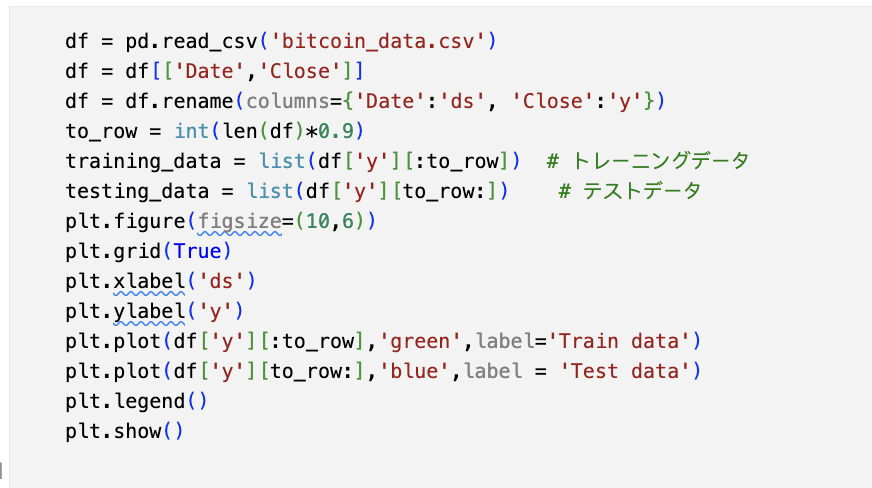
\includegraphics[keepaspectratio, scale=0.5]{pic/data_pre.png}
        \end{center}
    \end{figure}    
\end{frame}


\section{Prophet Model}
\subsection{Facebookが開発した時系列解析用のライブラリー}

\begin{frame}{Facebook Prophetモデルの設定}
    \begin{figure}[h]
        Facebook Prophetの時系列解析モデル\\
        (詳細: https://facebook.github.io/prophet/)
        \begin{center}
            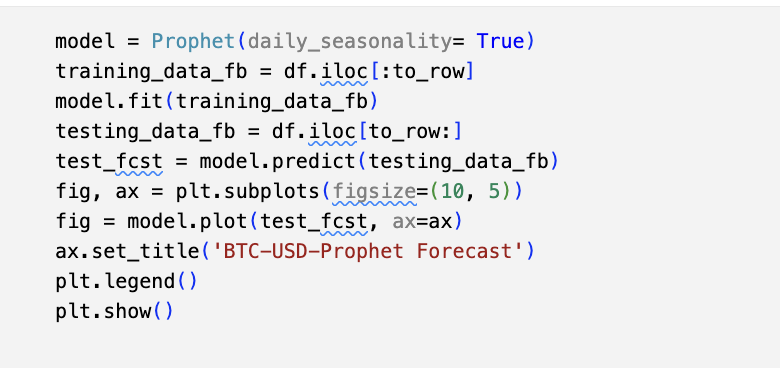
\includegraphics[keepaspectratio, scale=0.6]{pic/pp_set.png}
        \end{center}
    \end{figure}  
\end{frame}

\begin{frame}{一般化予測}
    \begin{figure}[h]
        \begin{center}
            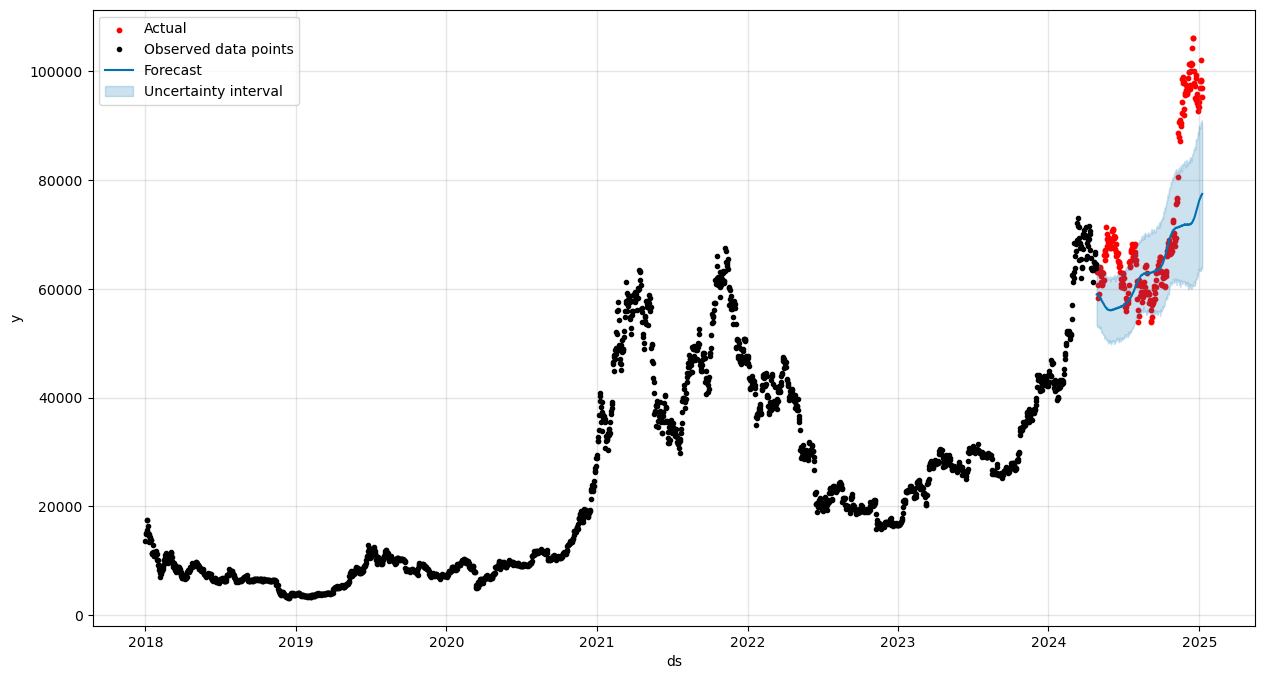
\includegraphics[keepaspectratio, width=0.5\textwidth]{pic/pp_fcst1_1.png}\\
            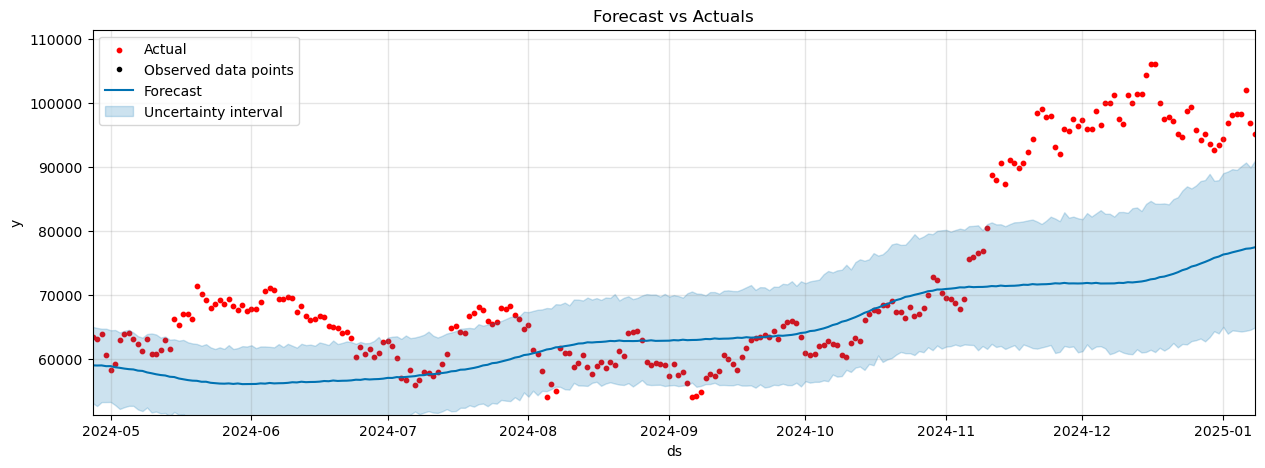
\includegraphics[keepaspectratio, width=0.6\textwidth]{pic/pp_fcst1_2.png}\\
            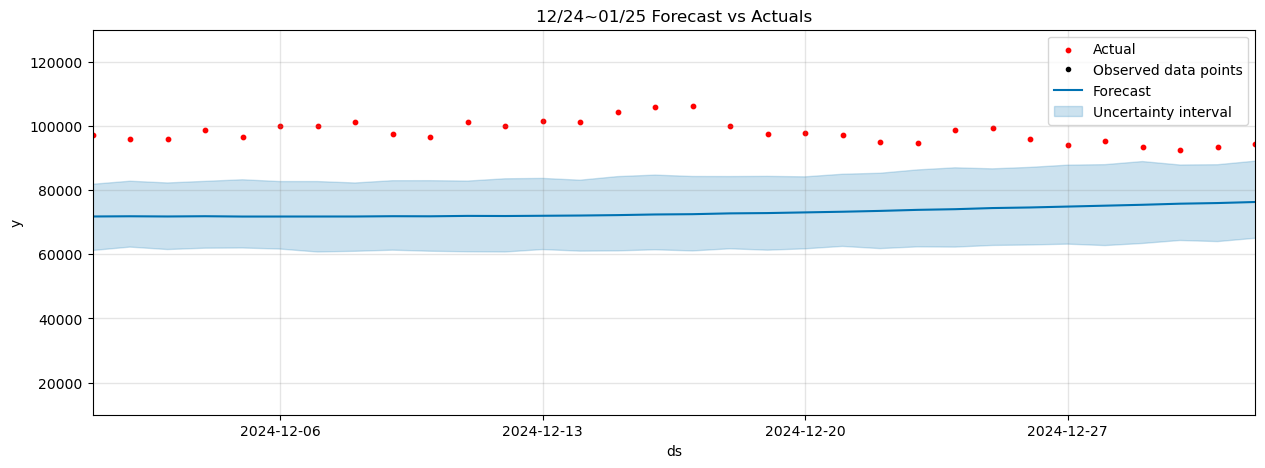
\includegraphics[keepaspectratio, width=0.6\textwidth]{pic/pp_fcst1_3.png}
        \end{center}
    \end{figure}
\end{frame}

\begin{frame}
    \frametitle{年月日のトレンド}
    \begin{figure}[h]
        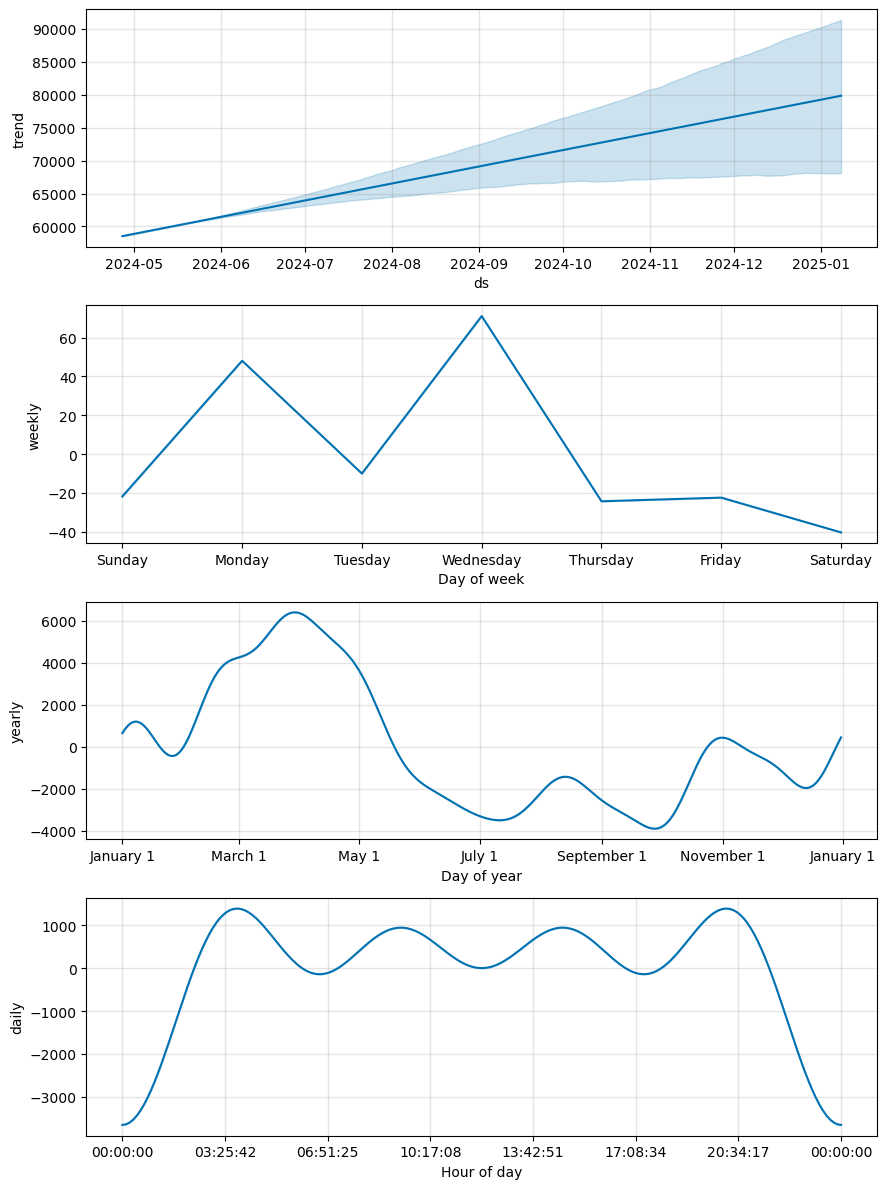
\includegraphics[keepaspectratio, width=0.5\textwidth]{pic/pp_fcst1.png}
    \end{figure}
\end{frame}

\begin{frame}
    \frametitle{モデルの評価}
\begin{itemize}
   \item  MSE Value(平均二乗誤差): 12724.452579794137\\
   \item  MAE Value(平均絶対誤差): 9289.974856441853\\
   \item  MAPE Value(平均絶対パーセント誤差): 11.582111797512047
\end{itemize}
\end{frame}

\begin{frame}
    \frametitle{祝日含みでのモデル訓練}
    \begin{figure}[h]
        \begin{center}
            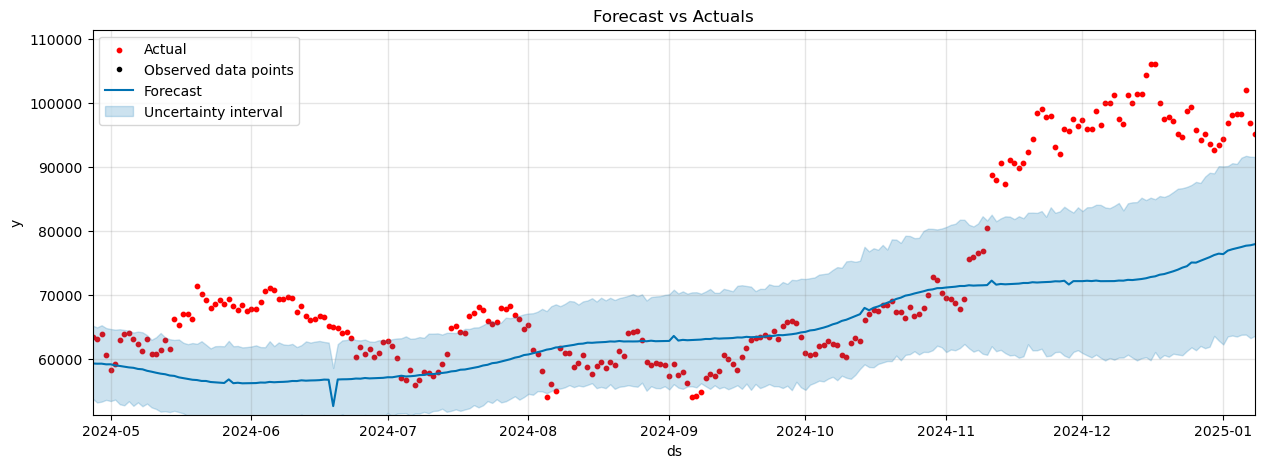
\includegraphics[keepaspectratio, width=0.65\textwidth]{pic/pp_fcst2_1.png}\\
            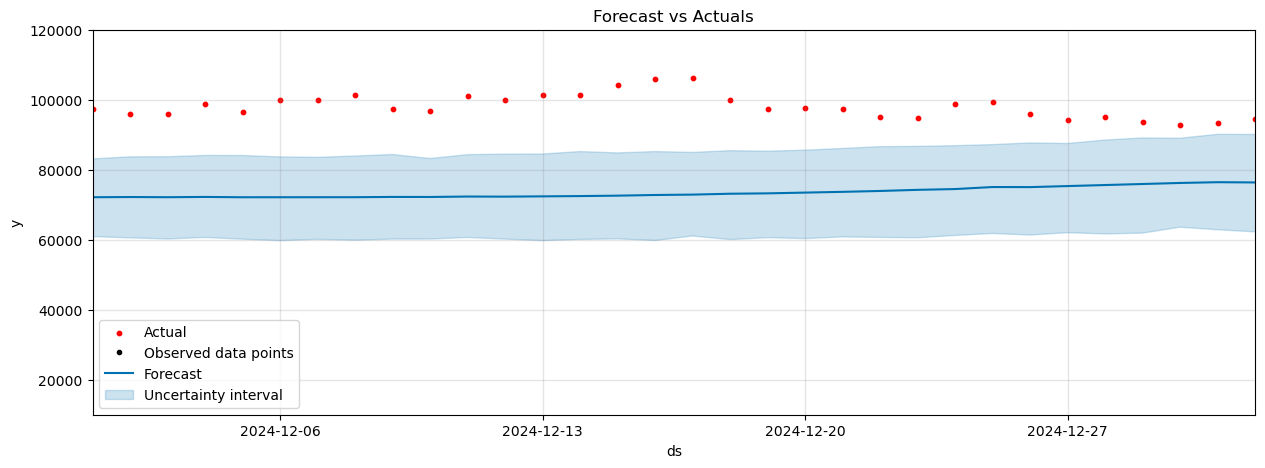
\includegraphics[keepaspectratio, width=0.65\textwidth]{pic/pp_fcst2_2.png}
        \end{center}
    \end{figure}
\end{frame}

\begin{frame}
    \frametitle{祝日含み版}
    \begin{figure}[htbp]
        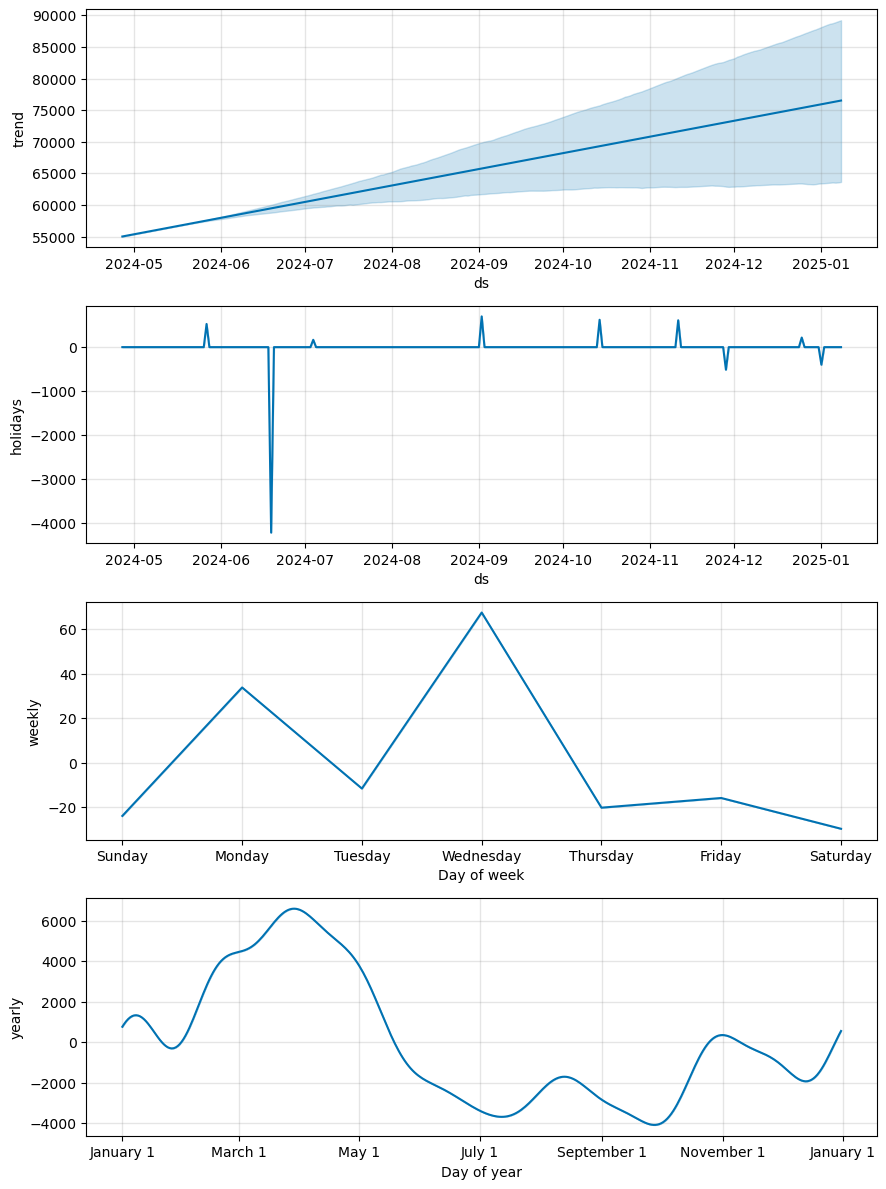
\includegraphics[keepaspectratio, width=0.6\textwidth]{pic/pp_fcst2.png}
    \end{figure}
\end{frame}

\begin{frame}
    \frametitle{祝日版Prophetモデル評価}
    \begin{itemize}
        \item SE Value(平均二乗誤差): 12550.97617585529
        \item MAE Value(平均絶対誤差): 9187.666839253901
        \item MAPE Value(平均絶対パーセント誤差): 11.468800365741414
    \end{itemize}
\end{frame}

\begin{frame}
    \frametitle{未来1年の予測}
    \begin{figure}[h]
        \begin{center}
            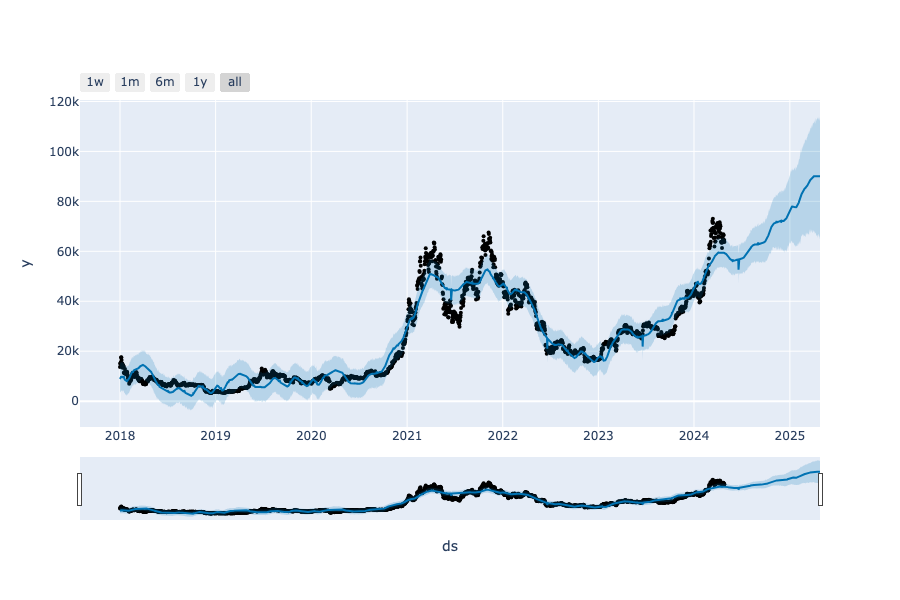
\includegraphics[keepaspectratio, width=0.95\textwidth]{pic/prophet_all.png}
        \end{center}
    \end{figure}
\end{frame}

\section{ARIMA Model}

\subsection{自己回帰和分移動平均モデル}

\begin{frame}
    \frametitle{訓練データとテストデータの大分け}
    訓練データ:全体データの0.9\\
    テストデータ:全体データ0.1
    \begin{figure}[h]
        \begin{center}
            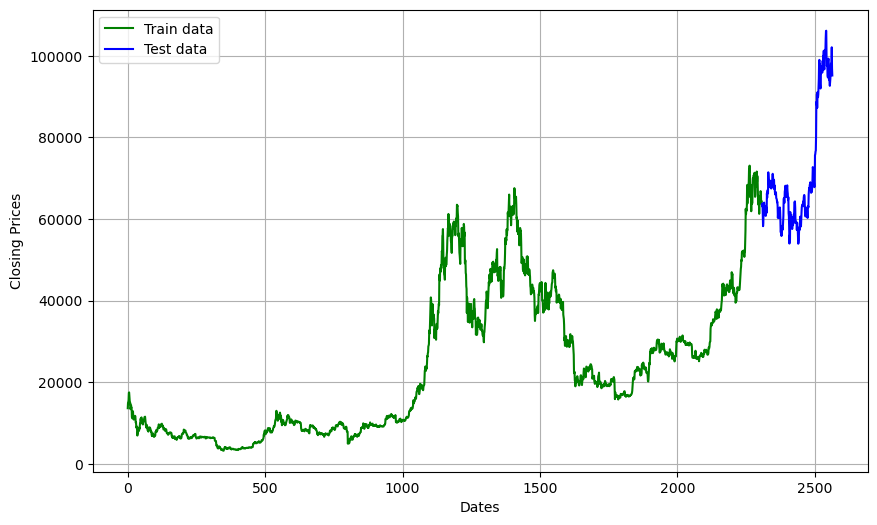
\includegraphics[keepaspectratio, width=0.95\textwidth]{pic/ar0.png}
        \end{center}
    \end{figure}
\end{frame}

\begin{frame}
    \frametitle{訓練したARIMAモデルとテストデータの対比}
    \begin{figure}[h]
        \begin{center}
            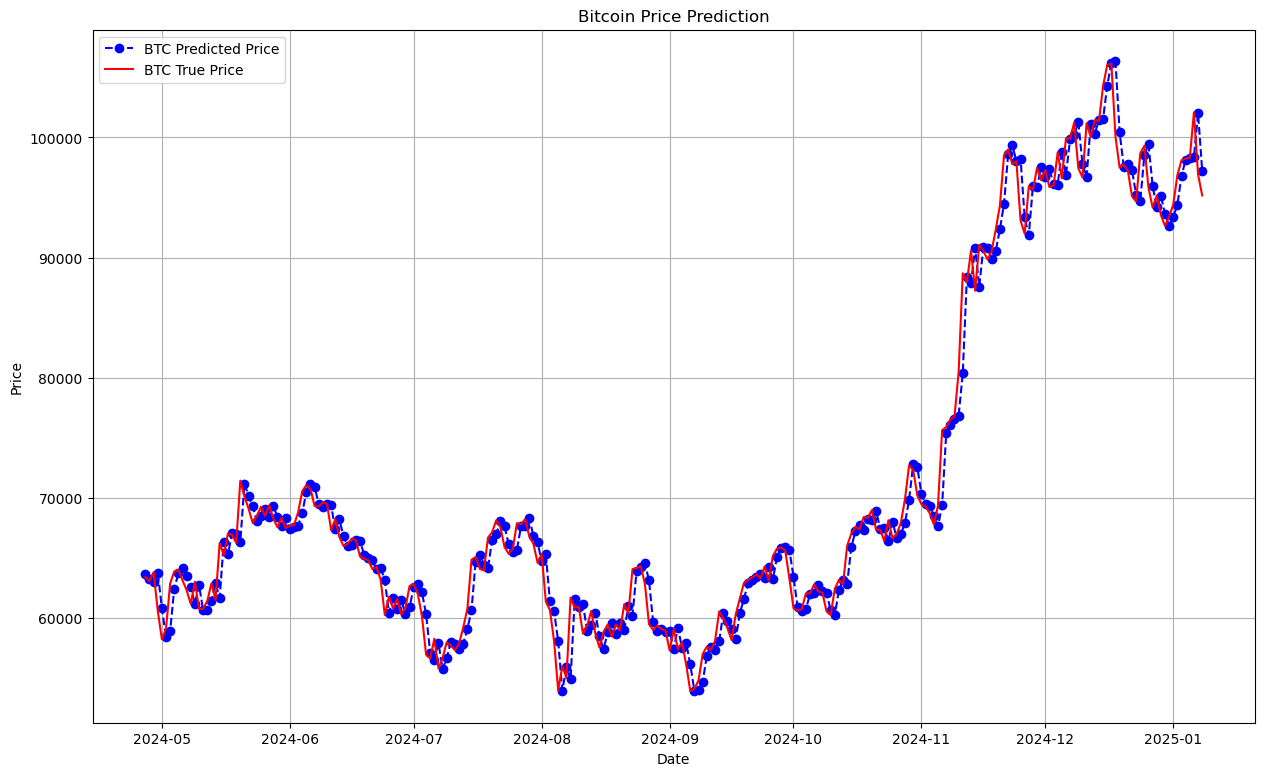
\includegraphics[keepaspectratio, width=0.95\textwidth]{pic/ar1.png}
        \end{center}
    \end{figure}
\end{frame}

\begin{frame}
    \frametitle{ARIMAモデルの評価}
    \begin{itemize}
        \item MAPE Value :1.94、すなわち、正確率は0.9806である
    \end{itemize}
\end{frame}


\begin{frame}
    \frametitle{ARIMAモデルでの未来1週間の価格予測}
    \begin{figure}[h]
        \begin{center}
            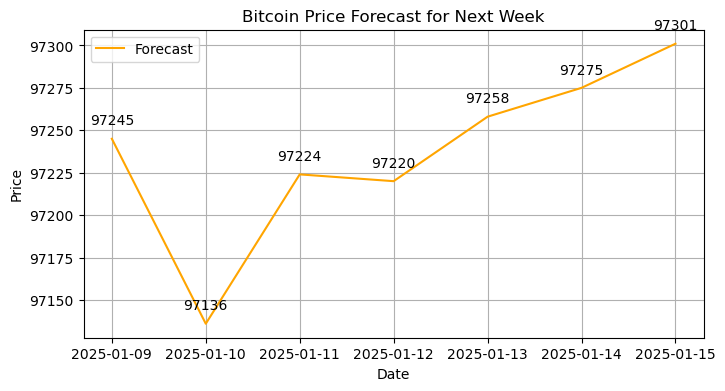
\includegraphics[keepaspectratio, width=0.95\textwidth]{pic/ar2.png}
        \end{center}
    \end{figure}
\end{frame}

\section{LSTM Model}

\subsection{ディープラーニング}
\begin{frame}
    \frametitle{データの標準化}
    \begin{figure}[h]
        \begin{center}
            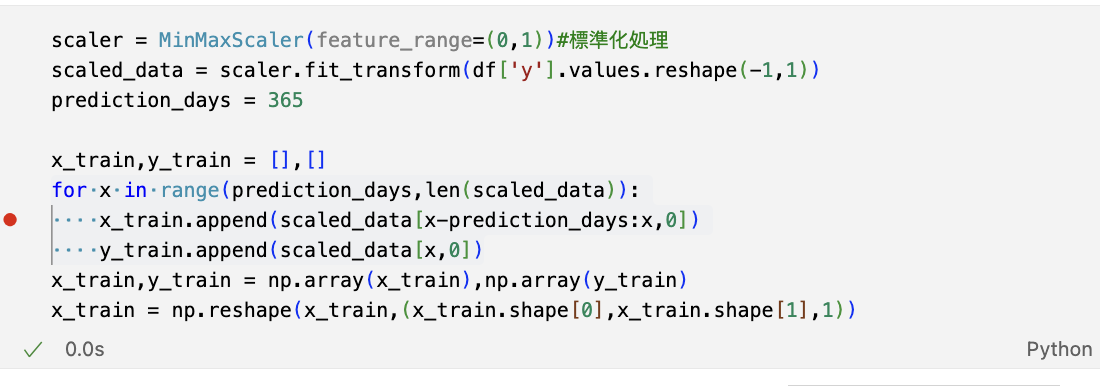
\includegraphics[keepaspectratio, width=0.95\textwidth]{pic/dl0.png}
        \end{center}
    \end{figure}
\end{frame}

\begin{frame}
    \frametitle{LSTMモデルの設定}
    \begin{figure}[h]
        \begin{center}
            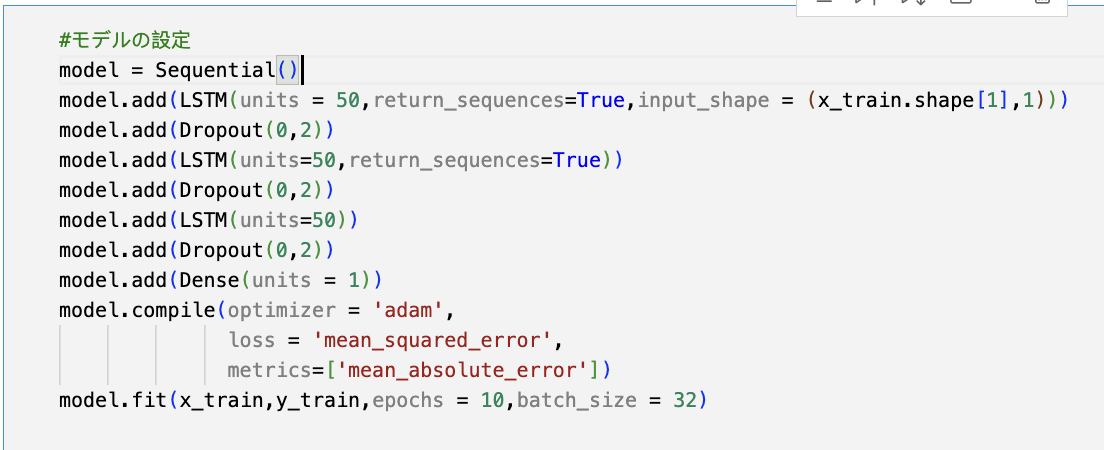
\includegraphics[keepaspectratio, width=0.95\textwidth]{pic/dl1.png}
        \end{center}
    \end{figure}
\end{frame}

\begin{frame}
    \frametitle{訓練したLSTMモデルとテストデータの対比}
    \begin{figure}[h]
        \begin{center}
            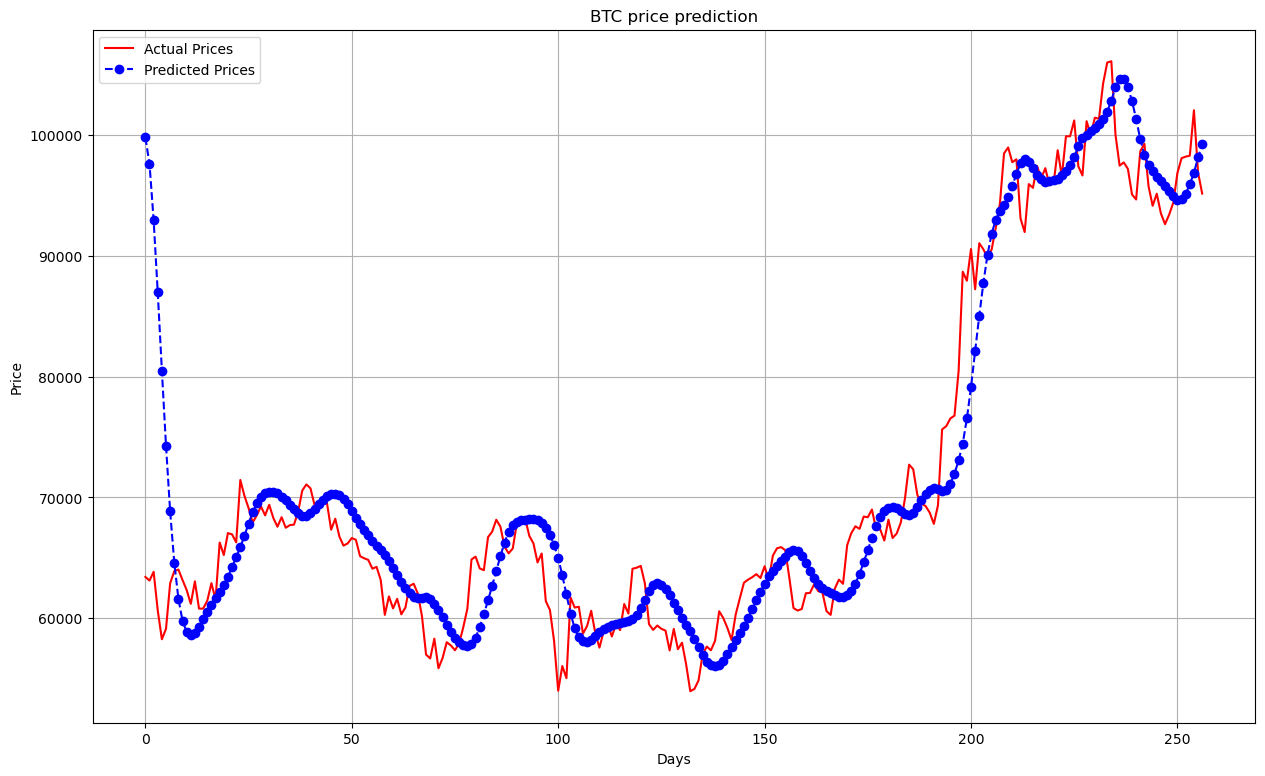
\includegraphics[keepaspectratio, width=0.95\textwidth]{pic/dl2.png}
        \end{center}
    \end{figure}
\end{frame}

\begin{frame}
    \frametitle{LSTMモデルの評価}
    \begin{itemize}
        \item MAPE Value:20、すなわち、正確率は0.8である
    \end{itemize}
\end{frame}

\section{References}
\begin{frame}
    \begin{itemize}
        \item Prophetモデルの紹介は(https://www.skillupai.com/blog/tech/prophet/#no1)を参考してください
        \item Prophetの原理は(https://zhuanlan.zhihu.com/p/463183142)とコードの原理(https://zhuanlan.zhihu.com/p/52330017)を参考してください
        \item ARIMAモデルの原理の紹介は(https://datastudy.gonna.jp/arima/)を参考してください
        \item LSTMモデルの紹介は(https://qiita.com/KojiOhki/items/89cd7b69a8a6239d67ca)を参考してください
    \end{itemize}
\end{frame}



% \begin{frame}{Algorithms}
%     \begin{exampleblock}{Non-Numbering Formula}
%         \begin{equation*}
%             J(\theta) = \mathbb{E}_{\pi_\theta}[G_t] = \sum_{s\in\mathcal{S}} d^\pi (s)V^\pi(s)=\sum_{s\in\mathcal{S}} d^\pi(s)\sum_{a\in\mathcal{A}}\pi_\theta(a|s)Q^\pi(s,a)% 公式放中间,不加公式番号(equation*)
%         \end{equation*}
%     \end{exampleblock}
%     \begin{exampleblock}{Multi-Row Formula\footnote{If text appears in the formula,use $\backslash$mathrm\{\} or $\backslash$text\{\} instead}}
%         \begin{align}
%             Q_\mathrm{target}&=r+\gamma Q^\pi(s^\prime, \pi_\theta(s^\prime)+\epsilon)\\
%             \epsilon&\sim\mathrm{clip}(\mathcal{N}(0, \sigma), -c, c)\nonumber
%         \end{align}
%     \end{exampleblock}
% \end{frame}

% \begin{frame}
%     \begin{exampleblock}{Numbered Multi-line Formula}% 演算公式
%         % Taken from Mathmode.tex
%         \begin{multline}
%             A=\lim_{n\rightarrow\infty}\Delta x\left(a^{2}+\left(a^{2}+2a\Delta x+\left(\Delta x\right)^{2}\right)\right.\label{eq:reset}\\
%             +\left(a^{2}+2\cdot2a\Delta x+2^{2}\left(\Delta x\right)^{2}\right)\\
%             +\left(a^{2}+2\cdot3a\Delta x+3^{2}\left(\Delta x\right)^{2}\right)\\
%             +\ldots\\
%             \left.+\left(a^{2}+2\cdot(n-1)a\Delta x+(n-1)^{2}\left(\Delta x\right)^{2}\right)\right)\\
%             =\frac{1}{3}\left(b^{3}-a^{3}\right)
%         \end{multline}
%     \end{exampleblock}
% \end{frame}

% \begin{frame}{Graphics and Columns}
%     \begin{minipage}[c]{0.3\linewidth}
%         \psset{unit=0.8cm}
%         \begin{pspicture}(-1.75,-3)(3.25,4)
%             \psline[linewidth=0.25pt](0,0)(0,4)
%             \rput[tl]{0}(0.2,2){$\vec e_z$}
%             \rput[tr]{0}(-0.9,1.4){$\vec e$}
%             \rput[tl]{0}(2.8,-1.1){$\vec C_{ptm{ext}}$}
%             \rput[br]{0}(-0.3,2.1){$\theta$}
%             \rput{25}(0,0){%
%             \psframe[fillstyle=solid,fillcolor=lightgray,linewidth=.8pt](-0.1,-3.2)(0.1,0)}
%             \rput{25}(0,0){%
%             \psellipse[fillstyle=solid,fillcolor=yellow,linewidth=3pt](0,0)(1.5,0.5)}
%             \rput{25}(0,0){%
%             \psframe[fillstyle=solid,fillcolor=lightgray,linewidth=.8pt](-0.1,0)(0.1,3.2)}
%             \rput{25}(0,0){\psline[linecolor=red,linewidth=1.5pt]{->}(0,0)(0.,2)}
% %           \psRotation{0}(0,3.5){$\dot\phi$}
% %           \psRotation{25}(-1.2,2.6){$\dot\psi$}
%             \psline[linecolor=red,linewidth=1.25pt]{->}(0,0)(0,2)
%             \psline[linecolor=red,linewidth=1.25pt]{->}(0,0)(3,-1)
%             \psline[linecolor=red,linewidth=1.25pt]{->}(0,0)(2.85,-0.95)
%             \psarc{->}{2.1}{90}{112.5}
%             \rput[bl](.1,.01){C}
%         \end{pspicture}
%     \end{minipage}\hspace{2cm}
%     \begin{minipage}{0.5\linewidth}
%         \medskip
%         % \hspace{2cm}
%         \begin{figure}[h]
%             \centering
%             \includegraphics[height=.4\textheight]{pic/sample.pdf}
%         \end{figure}
%     \end{minipage}
% \end{frame}

% \begin{frame}[fragile]{\LaTeX{} Common Commands}
%     \begin{exampleblock}{Commands}
%         \centering
%         \footnotesize
%         \begin{tabular}{llll}
%             \cmd{chapter} & \cmd{section} & \cmd{subsection} & \cmd{paragraph} \\
%             chapter & section & sub-section & paragraph \\\hline
%             \cmd{centering} & \cmd{emph} & \cmd{verb} & \cmd{url} \\
%             center & emphasize & original & hyperlink \\\hline
%             \cmd{footnote} & \cmd{item} & \cmd{caption} & \cmd{includegraphics} \\
%             footnote & list item & caption & insert image \\\hline
%             \cmd{label} & \cmd{cite} & \cmd{ref} \\
%             label & citation & refer\\\hline
%         \end{tabular}
%     \end{exampleblock}
%     \begin{exampleblock}{Environment}
%         \centering
%         \footnotesize
%         \begin{tabular}{lll}
%             \env{table} & \env{figure} & \env{equation}\\
%             table & figure & formula \\\hline
%             \env{itemize} & \env{enumerate} & \env{description}\\
%             non-numbering item & numbering item & description \\\hline
%         \end{tabular}
%     \end{exampleblock}
% \end{frame}

% \begin{frame}[fragile]{\LaTeX{} Examples of environmental commands}
%     \begin{minipage}{0.5\linewidth}
% \begin{lstlisting}[language=TeX]
% \begin{itemize}
%   \item A \item B
%   \item C
%   \begin{itemize}
%     \item C-1
%   \end{itemize}
% \end{itemize}
% \end{lstlisting}
%     \end{minipage}\hspace{1cm}
%     \begin{minipage}{0.3\linewidth}
%         \begin{itemize}
%             \item A
%             \item B
%             \item C
%             \begin{itemize}
%                 \item C-1
%             \end{itemize}
%         \end{itemize}
%     \end{minipage}
%     \medskip
%     \pause
%     \begin{minipage}{0.5\linewidth}
% \begin{lstlisting}[language=TeX]
% \begin{enumerate}
%   \item A \item B
%   \item C
%   \begin{itemize}
%     \item[n+e]
%   \end{itemize}
% \end{enumerate}
% \end{lstlisting}
%     \end{minipage}\hspace{1cm}
%     \begin{minipage}{0.3\linewidth}
%         \begin{enumerate}
%             \item A
%             \item B
%             \item C
%             \begin{itemize}
%                 \item[n+e]
%             \end{itemize}
%         \end{enumerate}
%     \end{minipage}
% \end{frame}

% \begin{frame}[fragile]{\LaTeX{} Formulas}
%     \begin{columns}
%         \begin{column}{.55\textwidth}
% \begin{lstlisting}[language=TeX]
% $V = \frac{4}{3}\pi r^3$

% \[
%   V = \frac{4}{3}\pi r^3
% \]

% \begin{equation}
%   \label{eq:vsphere}
%   V = \frac{4}{3}\pi r^3
% \end{equation}
% \end{lstlisting}
%         \end{column}
%         \begin{column}{.4\textwidth}
%             $V = \frac{4}{3}\pi r^3$
%             \[
%                 V = \frac{4}{3}\pi r^3
%             \]
%             \begin{equation}
%                 \label{eq:vsphere}
%                 V = \frac{4}{3}\pi r^3
%             \end{equation}
%         \end{column}
%     \end{columns}
%     \begin{itemize}
%         \item more information \href{https://ja.overleaf.com/learn/latex/Mathematical_expressions}{\color{purple}{here}}
%     \end{itemize}
% \end{frame}

% \begin{frame}[fragile]
%     \begin{columns}
%         \column{.6\textwidth}
% \begin{lstlisting}[language=TeX]
% \begin{table}[htbp]
%   \caption{numbers & meaning}
%   \label{tab:number}
%   \centering
%   \begin{tabular}{cl}
%     \toprule
%     number & meaning \\
%     \midrule
%     1 & 4.0 \\
%     2 & 3.7 \\
%     \bottomrule
%   \end{tabular}
% \end{table}
% \end{lstlisting}
%         \column{.4\textwidth}
%         \begin{table}[htpb]
%             \centering
%             \caption{numbers \& meaning}
%             \label{tab:number}
%             \begin{tabular}{cl}\toprule
%                 numbers & meaning \\\midrule
%                 1 & 4.0\\
%                 2 & 3.7\\\bottomrule
%             \end{tabular}
%         \end{table}
%         \normalsize formula~(\ref{eq:vsphere}) at previous slide and Table~\ref{tab:number}。
%     \end{columns}
% \end{frame}

% \section{Results}
% \begin{frame}
%     \begin{itemize}
%         \item \lipsum[4][1-4]
%         \item \lipsum[4][5-9]
%         \item \lipsum[5][1-4]
%         \item \lipsum[5][5-8]
%     \end{itemize}
% \end{frame}

% \section{References}

% \begin{frame}[allowframebreaks]
%     \bibliography{ref}
%     \bibliographystyle{ieeetr}
%     \nocite{*} % used here because no citation happens in slides
%     % if there are too many try use:
%     % \tiny\bibliographystyle{alpha}
% \end{frame}


% \begin{frame}
%     \begin{center}
%         {\Huge\calligra Thank You}
%     \end{center}
% \end{frame}

\end{document}